\section{Supporting Material}


\begin{figure}[ht!]
  \begin{minipage}{.49\textwidth}
    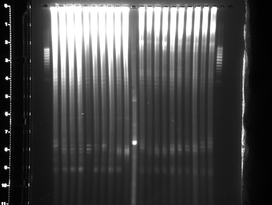
\includegraphics[width=\textwidth]{figures/diurnal/Y_CQ01_high_exposure.png}
  \end{minipage}
  \begin{minipage}{.49\textwidth}
    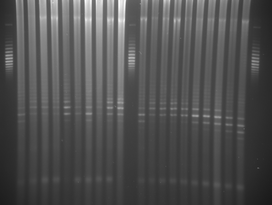
\includegraphics[width=\textwidth]{figures/diurnal/20130618_1511.png}
  \end{minipage}
  
  \vspace{-.5cm}
  \textbf{C}
  \vspace{.25cm}
  
  \begin{minipage}{.49\textwidth}
    
\includegraphics[width=\textwidth]{figures/diurnal/20130620_pCA_CQ1.png}
  \end{minipage}
  \begin{minipage}{.49\textwidth}
    
\includegraphics[width=\textwidth]{figures/diurnal/20130821_pCA_CQ20.png}
  \end{minipage}
  
  \vspace{-.5cm}
  \textbf{A}\hspace{.32\textwidth}\textbf{B}\hspace{.32\textwidth}\textbf{D}

  \caption{\textbf{Chloroquine Gel Analysis: Calibration \& Diurnal
      Supercoiling}. \small{\textbf{A \& B:} agarose gels of plasmid
      extracts from a diurnal growth experiments (see F); supplemented
      with \SI{1}{\ugml} (A) or \SI{20}{\ugml} (B) chloroquine
      diphosphate (CQ).  Additional lanes (left, right, center) show
      the pUC19 plasmid isolated from \textit{E.coli} cultures as a
      control, or (only A, central lane) a pooled plasmid sample after
      treatment with NcoI restriction enzyme which cuts only the
      pCA2.4\_M plasmid (one cut site) but not the similarly sized
      pCB2.4\_M. All topoisomer bands are replaced by a single band of
      linearized pCA2.4\_M. \textbf{C \& D:} Southern blots of the
      gels in (A) and (B) using probes specific for the pCA2.4\_M
      plasmid confirms the identity of the plasmid bands (Table
      \ref{tab:blot}).}}
    \label{fig:diurnalcq} 
\end{figure}


\begin{figure}
  \begin{minipage}{.27\textwidth}
    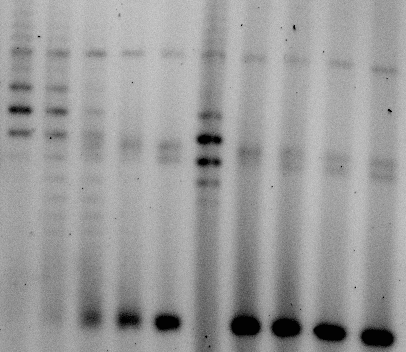
\includegraphics[width=\textwidth]{figures/diurnal/Y_CQ20_topoI_zoom_inv.png}
  \end{minipage}
  \begin{minipage}{.33\textwidth}
    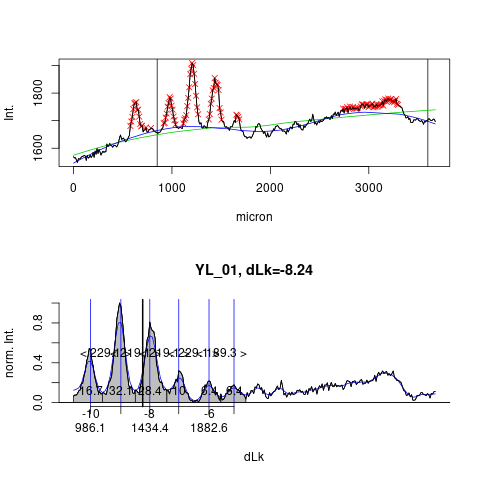
\includegraphics[width=\textwidth]{figures/diurnal/YL_01.png}
  \end{minipage}
  \begin{minipage}{.39\textwidth}
    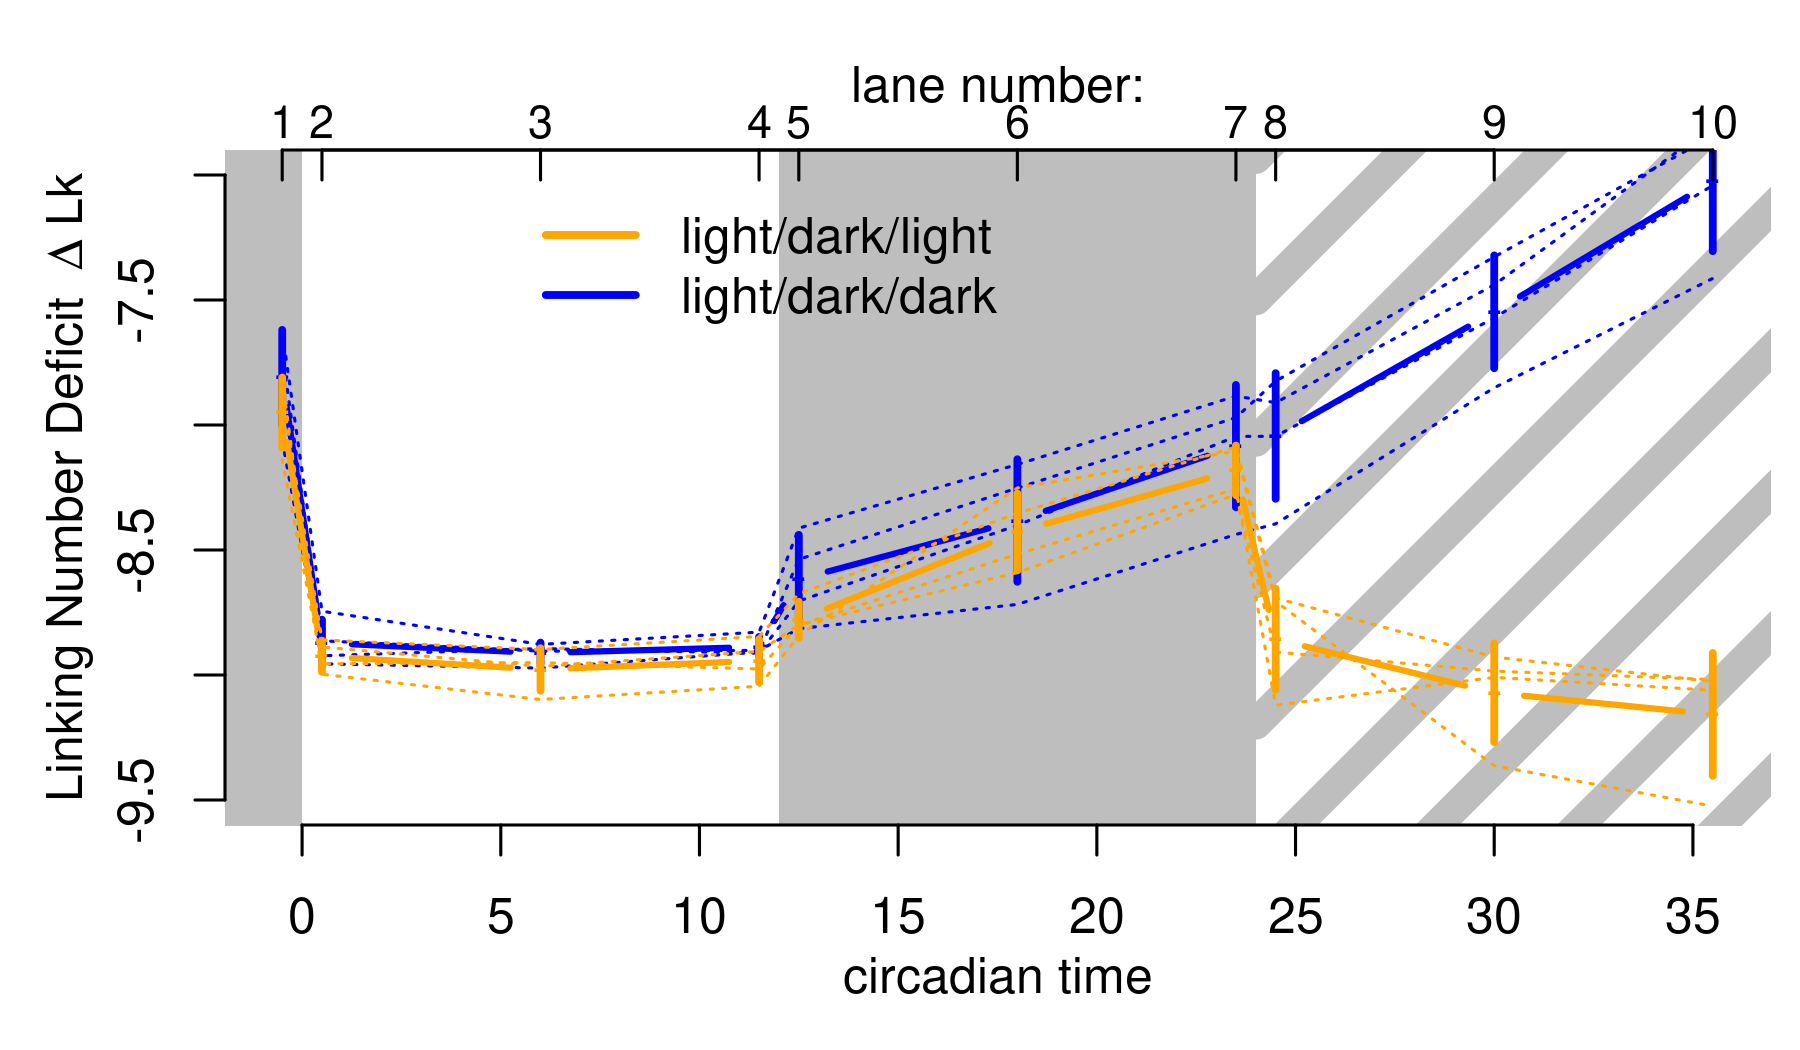
\includegraphics[width=\textwidth]{figures/diurnal/linkingNumbers.png}
  \end{minipage}
   
  \vspace{-.75cm}
  \textbf{A}\hspace{.26\textwidth}\textbf{B}\hspace{.33\textwidth}\textbf{C}
  \vspace{.25cm}
  
  \caption{\textbf{Chloroquine Gel Analysis: Calibration \& Diurnal
      Supercoiling}. \small{\textbf{A:} Mobility after relaxtion with
      topoisomerase I on an agarose gel with \SI{20}{\ugml} CQ
      confirms the faster migration of fully relaxed plasmids at these
      conditions. Lanes 1-5: plasmids from pooled light phase samples
      (YL). Lanes 6-10: plasmids from pooled dark phase samples
      (YD). The topoisomerase I reaction was run for 1, 5, 10 and 30
      min at \SI{37}{\celsius} (lanes 2-5, 7-10). The samples in lanes
      1 and 6 were treated as the 30 min samples, but did not contain
      topoisomerase I. \textbf{B:} Quantification of the linking
      number deficit $\Delta Lk$ for lane 2 (YL, 1 min) from
      electropherograms of the gel in (E).  See Methods for details;
      in short: a baseline was determined in two steps (top panel) and
      subtracted from the signal. For the range that included all
      topoisomers of interest (vertical lines in top panel) the
      location of peaks (bottom panel: vertical blue lines and x-axis
      annotation) was detected from a smoothed version of the signal
      (blue line). All peaks were assigned consecutive integral
      linking number values $\Delta Lk$ with an estimated offset from
      the relaxed form with $Lk=0$. The areas under the peaks
      $A_{\Delta Lk}$ were calculated (gray areas) and the average
      linking number deficit of the sample was then determined as the
      center of mass $\Delta \overline{Lk} = \sum{(\Delta Lk \cdot
        A_{\Delta Lk})}/\sum{A_{\Delta Lk}}$ of all topoisomer bands
      (thick black horizontal line and top axis
      annotation). \textbf{C:} Diurnal time-series of the average
      linking number deficits ($\Delta \overline{Lk}$) of the
      pCA2.4\_M plasmids, calculated from three replicates of the gel
      in Figure \ref{fig:diurnalcq}A and one replicate of the gel in
      \ref{fig:diurnalcq}B.  The dotted thin lines are values from
      the 4 different gels and the thick lines are their means and
      standard deviations.  Gray background indicates the dark
      phases. One culture (blue line, light/dark/dark) did not receive
      the final 12 h of light and remained in the dark.  Note, that
      lower values indicate more \textbf{negative} supercoiling
      (higher $|\Delta \overline{Lk}|$).}}
  \label{fig:topoi} 
\end{figure}

   
